\subsection*{3.1\quad 人工智能概述}

\begin{figure}[htbp]
\centering
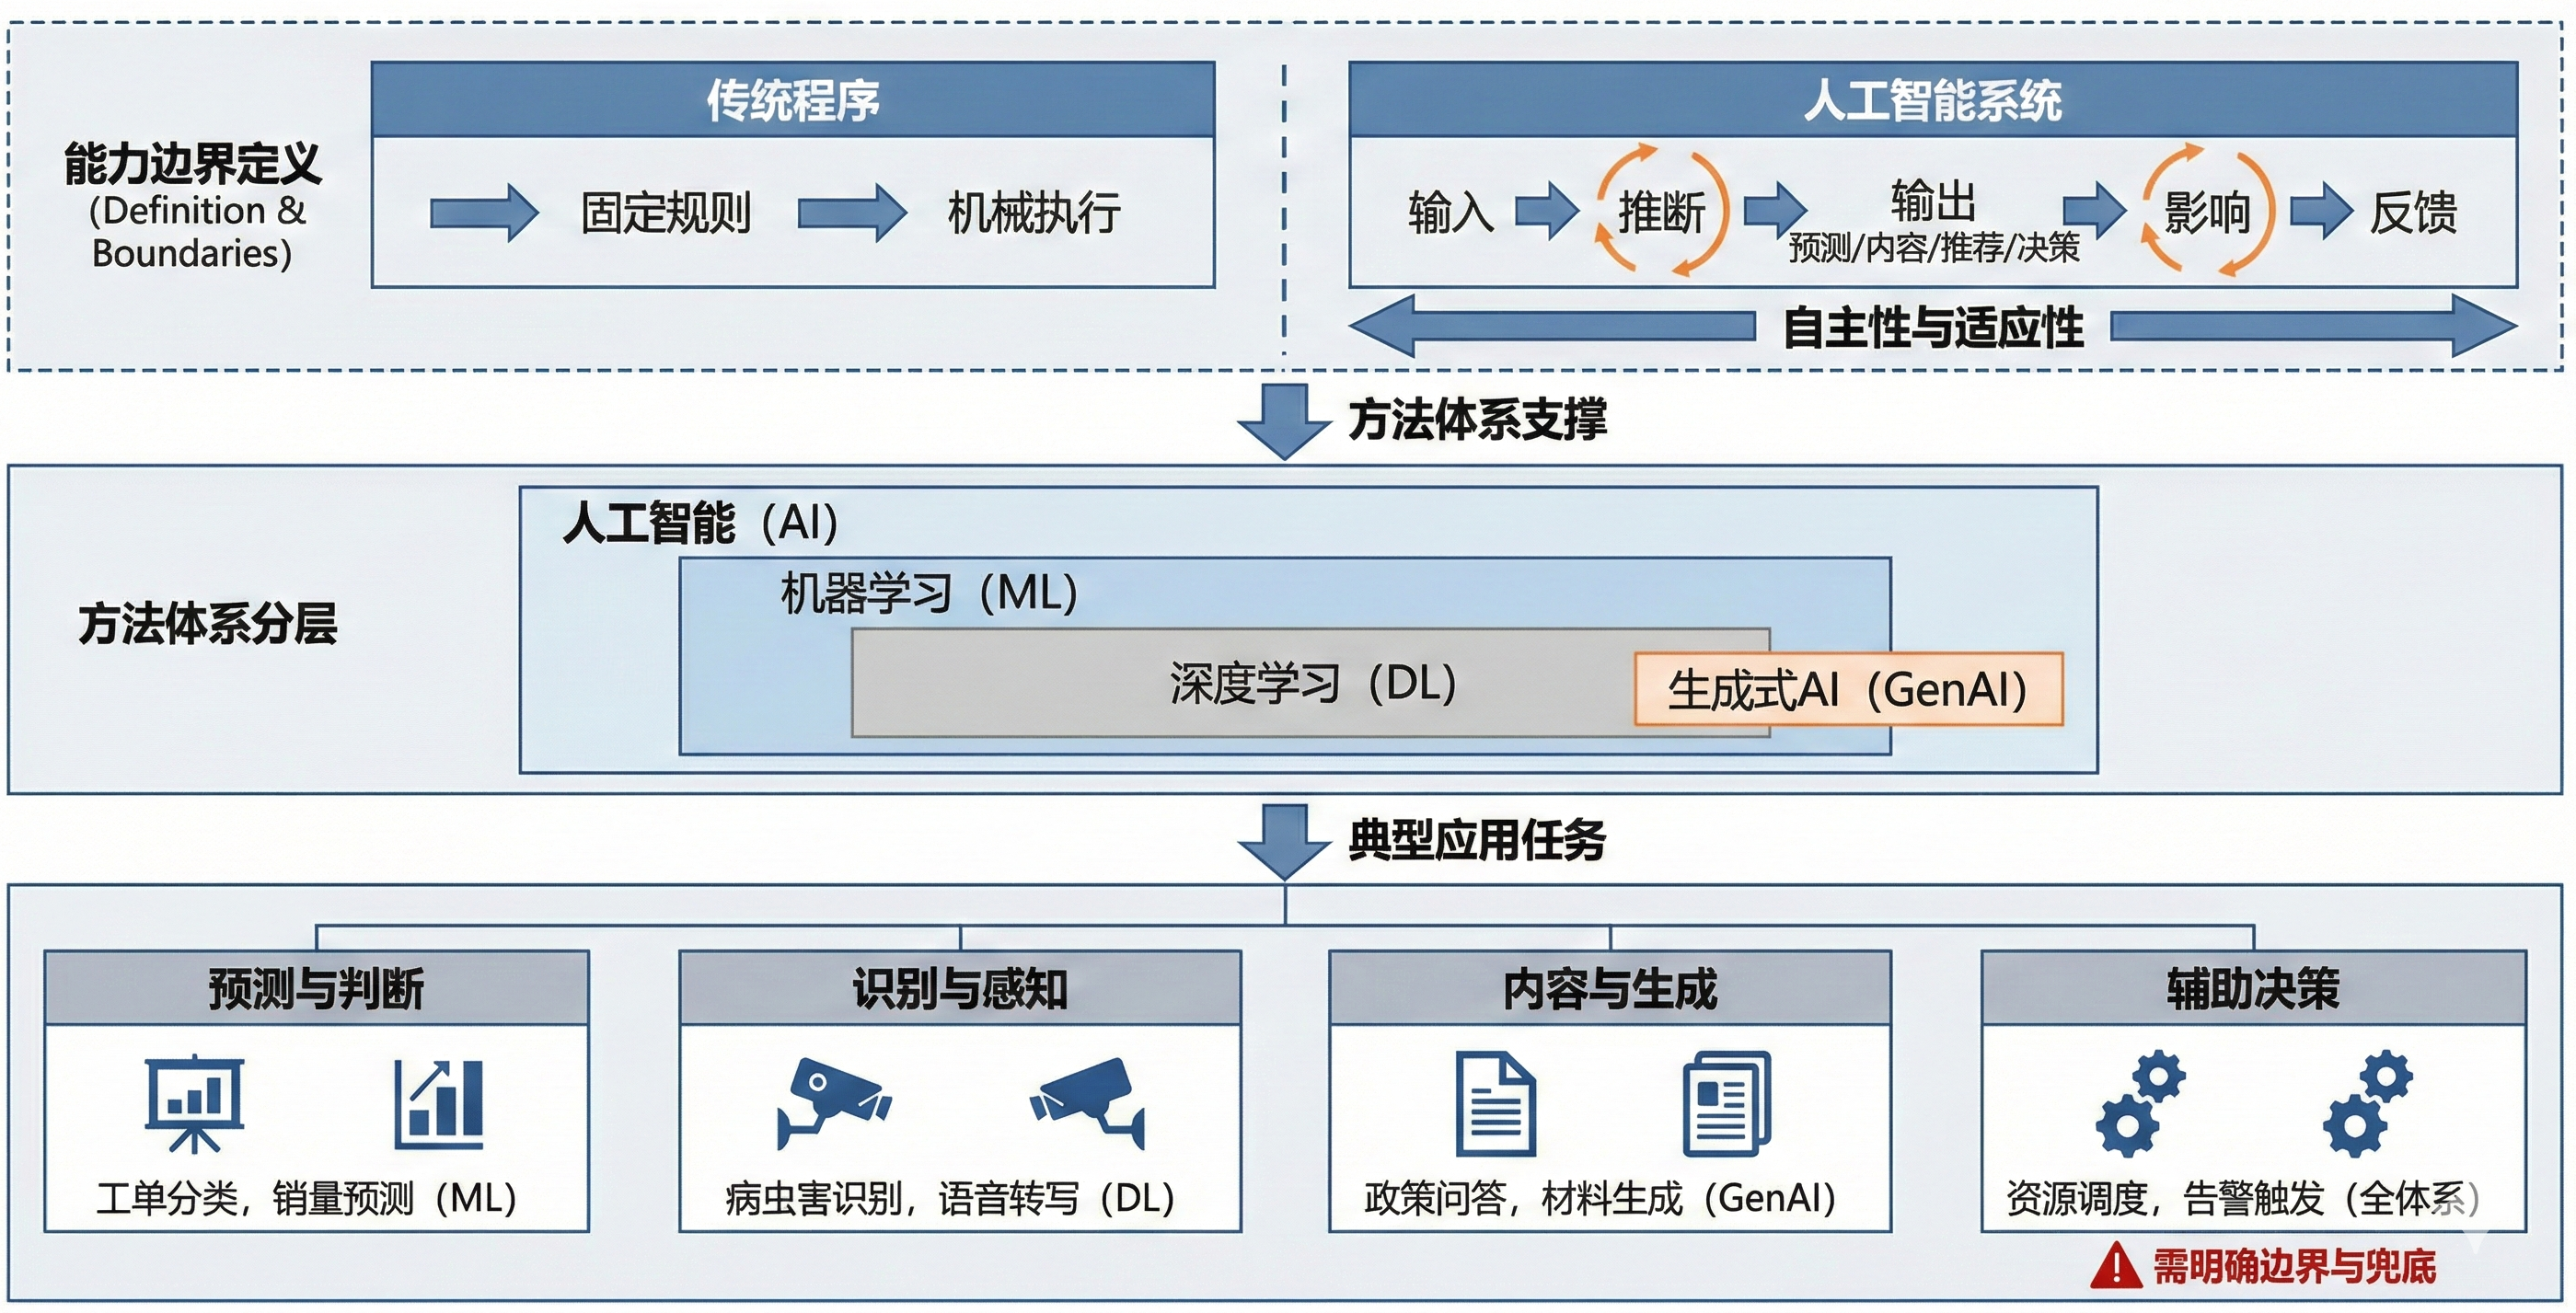
\includegraphics[width=0.9\textwidth]{figures/fig-ai-ml-dl-genai}
\caption{人工智能概念体系总览。}
\label{fig:ai-ml-dl-genai}
\end{figure}

\subsubsection*{3.1.1\quad 人工智能定义}
\noindent 人工智能是可工程化落地的系统,不是单一模型或单一功能。系统围绕明确或隐含的目标运行,从其接收的输入中进行推断,生成预测、内容、推荐或决策等输出,并且这些输出能够影响物理或虚拟环境。不同系统在自主性水平以及部署后的适应性方面存在差异。这样的表述强调目标、推断、输出、影响、自主与适应这一条可核对、可审计的链条,便于在跨学科沟通与项目交付中保持一致。

\noindent 这里所说的机器系统,并不等同于机器人设备,而是指能够被工程化实现并在一定规则与约束下运行的系统形态。它可能是纯软件系统,如热线工单分派、政策问答与材料清单生成,也可能是软硬一体的系统,如带摄像头的分拣设备、巡检终端或无人机采集与识别系统。之所以强调系统,是因为人工智能落地的成败通常不取决于某个模型的单点表现,而取决于数据来源与口径、流程嵌入方式、权限边界、人工复核与上线监控等要素是否形成闭环。这些要素共同决定系统输出能否稳定地支持业务动作。

\noindent 目标需要被明确区分为显式与隐含两类。显式目标是写入需求说明或指标体系的目标,如将工单按类别准确分派、降低备货浪费、缩短平均响应时长。隐含目标则是系统在运行中可能默认追求的方向,如尽可能提高点击率或响应速度。目标并非中性技术参数,它会直接牵引数据收集、模型优化方向与业务风险边界。同一套数据与技术在不同目标约束下可能导向完全不同的行为结果。因此目标的设定与约束首先是治理与管理问题,其次才是技术实现问题。

\noindent 从输入中进行推断是区分人工智能系统与一般自动化的关键。推断意味着系统不是机械复制输入或执行固定模板,而是基于规则、知识或数据训练得到的模型,对输入进行处理并形成对输出的判断。换言之,系统能够在一定范围内把既有经验迁移到新样本、新情形上,给出可重复、可检验的输出。反过来,如果某个流程仅是固定规则的机械串联,无推断机制,也不具备对新情况的处理能力,那么更适合被称为流程自动化,而不宜泛化称作人工智能。这种边界澄清的目的不是抬高门槛,而是为后续方法选择、效果评估与责任划分提供共同语言。

\noindent 在输出层面,将预测、内容、推荐、决策四类输出写清楚,可以把抽象能力直接对齐到业务动作。预测对应对未来或未知量的估计,如客流、销量、价格、病害风险。内容对应表达性输出,如宣讲稿、摘要、海报文案、材料清单整理。推荐对应候选项的排序或匹配,如政策匹配、课程推荐、资源配置建议。决策则对应触发动作或给出选择,如是否告警、是否进入人工复核、是否进入加急流程。只要输出能够影响物理或虚拟环境,就必须进一步讨论责任、边界与可追溯性。输出如何进入业务流程、由谁确认、如何留痕、如何纠错,决定了系统是辅助还是替代,也决定了风险控制的最低配置。

\noindent 最后,自主性与部署后的适应性用于刻画系统运行方式与风险管理强度。自主性越高,系统越可能在较少人工介入下连续运行。适应性越强,系统越可能在上线后根据新数据或新交互调整行为。一般而言,这两项能力越强,潜在效率收益越大,但对监控、审计、权限控制、阈值策略与兜底机制的要求也越高,且需要更明确地界定系统输出的可用范围与人应当介入的触发条件。

\noindent 放在乡村经营语境中,可以用一个最小案例把上述链条落到业务上。以政务热线工单分派为例,系统接收群众留言、地点与历史工单信息,通过推断识别问题类别与紧急程度,输出分派部门与响应时限,并据此影响工单流转、人员调度与现场处置。这个过程之所以可被称为人工智能系统,不在于它是否使用了复杂模型,而在于它围绕目标形成了从输入到输出的推断机制,并且输出被嵌入到可追溯、可纠错的业务流程之中。

\subsubsection*{3.1.2\quad 人工智能、机器学习、深度学习与生成式AI的区别}
\begin{figure}[htbp]
\centering
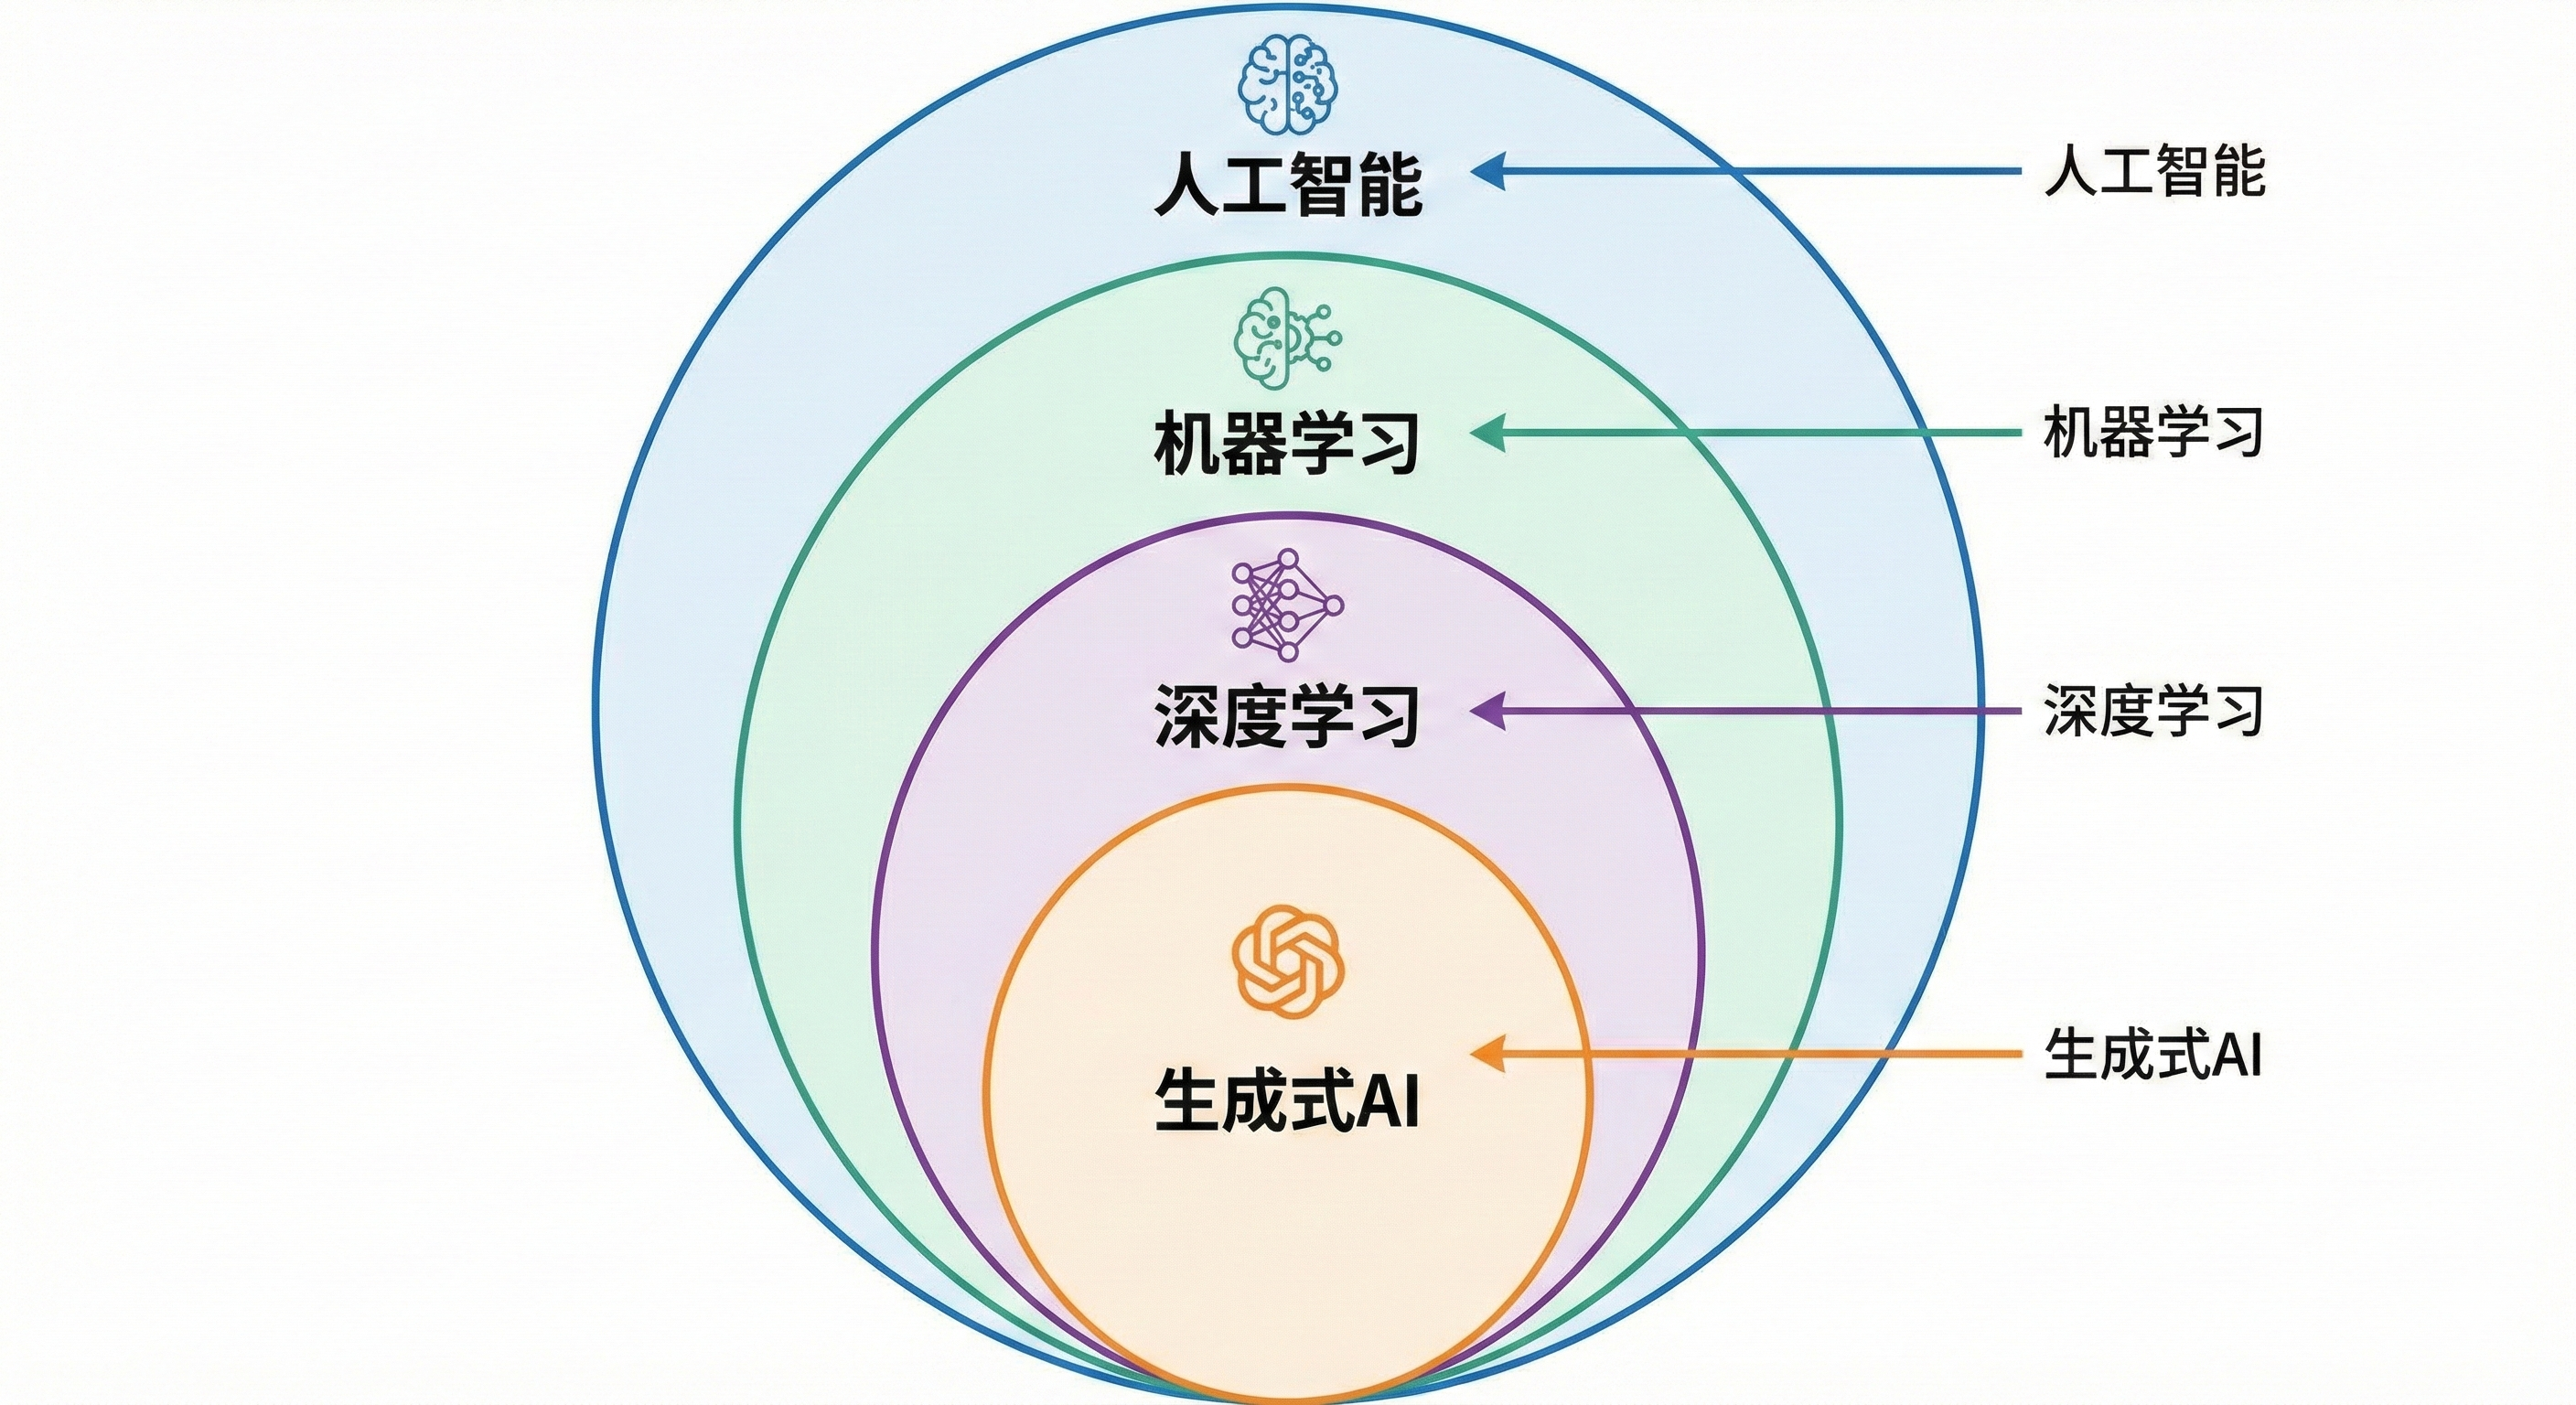
\includegraphics[width=0.9\textwidth]{figures/fig-ai-concept-hierarchy}
\caption{人工智能、机器学习、深度学习与生成式AI的概念层级与区别。}
\label{fig:ai-concept-hierarchy}
\end{figure}

\noindent 人工智能是总称,关注的是机器系统是否以目标为导向,能够基于输入进行推断并产生输出,且该输出能够影响物理或虚拟环境。系统之间在自主性与部署后适应性方面存在差异。这里强调系统,意味着人工智能并非等同于某个模型或某段代码,而是由数据、规则或模型、流程、权限、人工复核与监控等要素共同构成的业务机制。因而在乡村经营中,许多高价值的智能化并不依赖复杂模型,例如通过规则与流程实现的工单分派、资格初筛、风险分级,只要其输出是围绕明确目标形成的、可重复使用并能在一定范围内泛化到新情况的推断结果,就属于人工智能系统在业务链条中的一种实现方式。

\noindent 机器学习是人工智能的一条重要实现路径,其核心在于从数据中学习可泛化的映射关系。工程上,机器学习用训练数据把输入与输出之间的关系固化为模型,使系统能够在未见样本上进行预测或判断。管理上,它意味着用数据与统计规律替代部分人工经验与手写规则,从而在不确定环境中输出概率性或统计意义上的结论。机器学习尤其适合乡村经营中大量结构化数据场景,如台账与交易记录、客流与销量序列、工单与满意度指标等,因为这些数据容易形成稳定的字段口径、明确的评价指标与可持续迭代的反馈闭环。

\noindent 深度学习是机器学习的子集,其典型优势来自多层表示学习。系统能够在训练中自动学习从低层特征到高层语义的表示,降低对人工特征设计的依赖。这使其在图像、语音、文本等非结构化数据上更具竞争力,但也通常意味着更高的数据规模要求、更显著的标注与训练工程成本,以及更强的算力与运维能力约束。对乡村场景而言,凡是输入以图片、语音或长文本为主且模式复杂的任务,深度学习更常见,例如病虫害识别、分级分拣与遥感解译,访谈语音转写与结构化归档,以及长政策文本的要点抽取与归纳等。

\noindent 面对不同任务应结合目标、数据与流程约束选择相应的人工智能方法,确保效果、成本与风险可控。当目标是预测或判断,且数据主要呈现为表格台账与结构化字段时,优先采用机器学习,通常成本更可控、评估更清晰、上线更稳定。当输入以图片、语音或长文本为主且任务复杂、传统特征工程难以奏效时,再考虑深度学习,并在立项阶段同步评估标注成本、算力资源与运维能力。当目标是表达、整理、生成或对话,并且业务流程能够容纳引用约束与人工核验时,才考虑生成式AI,并将核验与权限边界作为交付验收项。至于系统输出直接触发资源分配、资金发放、执法处置等自动决策型应用,应在目标定义、权限控制、审计记录、风险阈值与兜底机制明确之后再推进,避免把模型判断或生成内容直接等同为可追责决策。

\subsubsection*{3.1.3\quad 人工智能与传统程序}
\noindent 传统程序把业务规则写进代码里,系统按既定流程执行。学习型系统把一部分规则交给数据与训练过程,让模型从样本中学出规律,再对新输入做出推断。这种差异决定了两类系统在建设方式、评估方式与风险控制上都不一样。

\noindent 传统程序要改得更好,通常是补规则、改代码、加校验,再通过测试上线。学习型系统要改得更好,通常要先把数据口径和标注方式理顺,再训练、评估、上线观测并持续迭代。它的输出往往带有概率性,需要用指标、阈值、人工复核与留痕来保证可用。

\noindent 规则清晰、责任边界要求严格、变化不大的流程更适合传统程序,例如资格条件明确的审核初筛、台账字段校验与流程提醒。规则难穷举、输入复杂或变化快的任务更适合学习型方法,例如工单分派中的类别识别、图片中的病虫害识别、长文本中的要点抽取与归纳。

\noindent 选型时可以先问一个问题,关键规则能不能写清楚并覆盖大多数情况。能写清楚且长期稳定就优先采用规则与流程自动化,写不清楚或需要从大量历史数据里找规律就考虑机器学习或深度学习。

\noindent 学习型系统也会带来新的代价,包括数据采集与标注成本、训练与运维成本、解释性与稳定性下降的风险。项目评审除了看效果,还要看数据来源是否可靠、指标是否可监控、上线后是否能持续维护与纠偏。

\begin{table}[h]
\centering
\caption{学习型系统与传统程序的对照}
\begin{tabular}{@{}llllll@{}}
\toprule
知识来源 & 开发方式 & 改进方式 & 适用输入 & 可解释性 & 部署维护 \\ \midrule
规则与流程 & 编写规则 & 改规则和改代码 & 结构化为主 & 高 & 相对稳定 \\
数据与训练 & 训练模型 & 数据和训练迭代 & 复杂与非结构化 & 中等或较低 & 需持续监测 \\ \bottomrule
\end{tabular}
\end{table}
